\chapter{Vehicle Semantics Extraction}

\label{section:semanticsextraction}


\section{Introduction}

In this chapter, the implementation of the vehicle semantic extraction module is discussed in detail. First, the process to separate the background and the objects of interest is discussed briefly in Section \ref{subsection:fundamental}. 
%Next, the atom-based quantization and database schema is introduced for both the \versionOne and \versionTwo based framework in Section \ref{section:dbschema}. 
Next, both the vehicle semantic extraction modules can then be thoroughly described in Section \ref{section:semantic_lsh} and Section \ref{section:semantic_chamfer}.


%While the implementation and adoption of the work proposed in \cite{lim2017} enabled the identification of moving objects from the background image, these information were not saved anywhere. First, a database schema was drawn out to determine the types of information that could be extracted from these foreground objects. Next, 



As describe in Section \ref{subsec:scope}, the two major semantics extracted in the proposed algorithm are (i) Vehicle Color and (ii) Vehicle Trajectory. Other semantic information such as the time and date which were extracted will not discussed in detail as these are simple extraction based on the input file names.


\section{Related Literature?}

what is semantics


\section{Fundamental Framework}
\label{subsection:fundamental}

Before the video dataset can be channelled to the vehicle semantics extraction, some pre-processing work has to be done. The fundamental framework was adopted from a portion of the work done by \cite{lim2017} where the author developed a framework to detect moving objects in a video using popular techniques such as background subtraction was applied to differentiate between static background and moving objects as depicted in Figure \ref{fig:bgs}. 

\begin{figure}[htb!]
  \centering
\begin{tabular}{cc}
 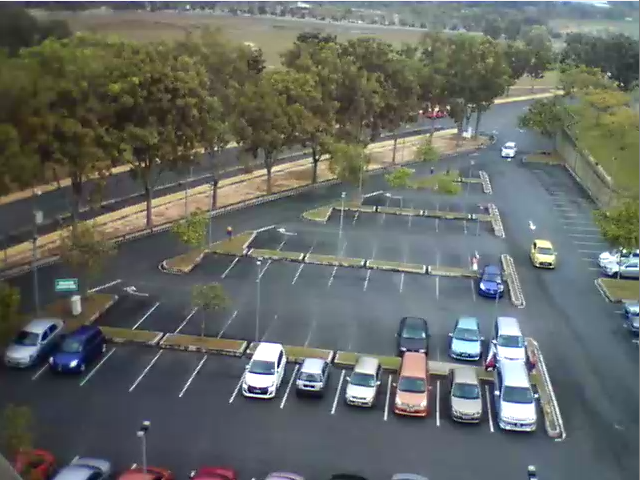
\includegraphics[width=0.4\linewidth]{image/general/bgs1.png} &  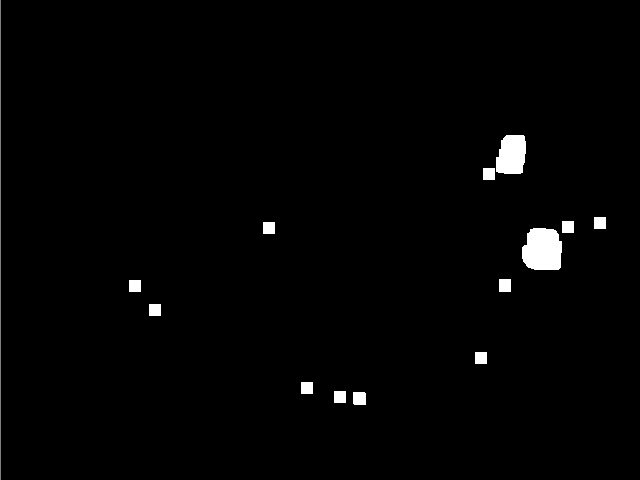
\includegraphics[width=0.4\linewidth]{image/general/bgs2.png}  \\ 
(a) 123th frame of a video & (b) Result of background subtraction \\
\end{tabular}
\caption{Background Subtraction} 
\label{fig:bgs}
\end{figure}

As the vanilla application of background subtraction often results with noisy output, the proposed algorithm used in \cite{lim2017} implemented a combination of adaptive learning and frame differencing method. This step was used to detect and extract moving objects (foreground blobs). This is then followed by several erosion and dilation morphology operators to further reduce the noise and to provide a better foreground blob at the end of the process.

\begin{figure}[htb!]
  \centering
\begin{tabular}{ccc}
 
\includegraphics[width=0.2\linewidth]{image/general/morph_ori.png} &  
\includegraphics[width=0.2\linewidth]{image/general/morph_erode.png} &
 
\includegraphics[width=0.2\linewidth]{image/general/morph_dilate.png}\\ 
(a) Original Image & (b) Eroded Image & (c) Dilated Image \\
\end{tabular}
\caption{Morphology Operations: Erosion \& Dilation} 
\label{fig:morph}
\end{figure}

The process is known as \textit{Opening} occurs when the morphology operations are done in the following sequence - 1) Erosion, \& 2) Dilation, noisy data from the background subtraction method can be eliminated as the erosion operation will be able to remove noise while maintaining the important subjects. In contrast, the operation known as \textit{closing} occurs when the dilation step is first performed, followed by the erosion step. This process is useful to fill up the gaps within the foreground objects. These processes are illustrated in Figure \ref{fig:morph2}

\begin{figure}[htb!]
  \centering
\begin{tabular}{cc}
 
\includegraphics[width=0.4\linewidth]{image/general/opening.png} &  \includegraphics[width=0.4\linewidth]{image/general/closing.png}  \\ 
(a) Opening & (b) Closing \\
\end{tabular}
\caption{Morphology Operations: Opening \& Closing} 
\label{fig:morph2}
\end{figure}


\cc{do i need to cite these images? \\}
%https://docs.opencv.org/3.0-beta/doc/py_tutorials/py_imgproc/py_morphological_ops/py_morphological_ops.html


Now with the background subtraction operation in place, the foreground objects can now be detected. Each of these foreground object are referred to as a \textit{blob}. Each of these blobs are then filtered using some handcrafted parameters to separate between vehicles and non-vehicles objects. To further enhance this process, a deep learning model was deployed to increase the probability of filtering non-vehicle blobs. 

In the proposed method pipeline, the work of \cite{redmon2016you} namely YOLOv2 (You Only Look Once) - a deep learning model was deployed as a complementary module. Now, as YOLO is a deep learning model designed to be real-time object detection, the detection process incurred very little overhead to the overall computational time and cost. Here, the bounding box of each foreground blob is sent into the YOLO network as an input. The network will then divide the input into multiple smaller regions and perform prediction of the bounding box along with the class probability. As the YOLO model is pre-trained with "vehicle" as one of the many classes, no further retraining was done in the proposed method pipeline.

With that in place, each of the blobs which were identified as a vehicle were tracked, on the other hand, blobs which were not identified as a vehicle was left as a possible candidate. This is done in view of misidentification due to poor lighting conditions or error during the background subtraction process. For each of the vehicle blobs, the semantic extraction module can now proceed.  


\section{Atom-based Quantization}
\label{section:atoms}

As the utilization of video data is the central focus in this work, there was a need for coming up with a way to easily manipulate and represent the video information. As video data can be commonly represented using the 3 dimensional space (X-axis, Y-axis, \& time-axis), there was an opportunity to convert the continuous data into discrete data blocks.     


In order to design a framework for large-scale extraction and retrieval of video semantics, this work adopted the concept of "atoms" as coined by \cite{castanon2016retrieval} which enabled quantization of the video input into individual 3D spatial-temporal cubes which consist of the X-axis, Y-axis and T-axis. In this work, an atom is defined as a group of cells at a similar spatial location, that spans a certain fixed number of frames; hence forming a spatio-temporal `cube'.

As described in Section \ref{section:dataset_used}, the input video data has a resolution of 640$\times$480 pixels and frame rate of 10$fps$, the dimensions of each atoms ($\alpha$) were analytically set to $\alpha_{width}=32$ pixels, $\alpha_{height}=24$ pixels and $\alpha_{time}=10$ frames, which represents the temporal duration of one second. The resolution of the atom ($\alpha_{width},\alpha_{height}$) were set as such so that the video resolution can be uniformly divided by 20 atoms across both its width and height as illustrated in Figure \ref{fig:viewfromcamera}. Hence, with this setup, each atom can be uniquely identified using the $X, Y$ and $T$ identifiers.



\begin{figure}[hbt!]\centering
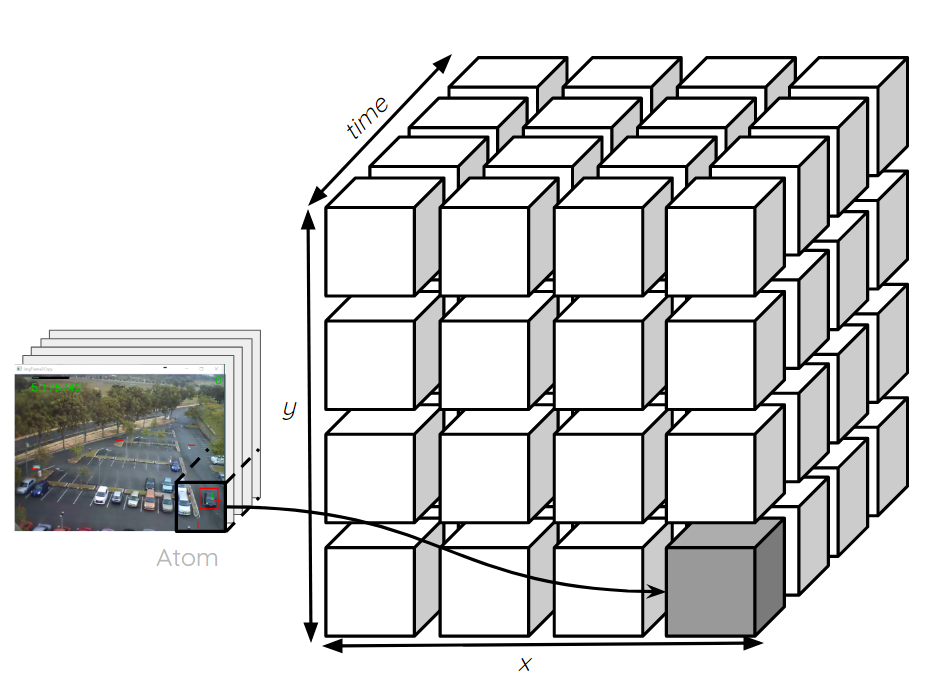
\includegraphics[width=.7\textwidth]{image/general/atom.PNG}
\caption{Quantization of Video Data into Atoms}
\label{fig:atoms}
\end{figure}

The use of these atom-based spatial-temporal cube is paramount in this work. By applying the quantization of data in the X,Y and T-axis, the atom-based structure enables two major types of queries to be performed conveniently. Figure \ref{fig:typesofQuery} illustrates the types of queries which are regularly desired when working with video data: Region of Interest (ROI) query \& Time-slicing query. More often than not, the queries used in real world applications are in the form of a combination of both the ROI and time-slicing query where the users are interested in certain activity that occured in a particular location given a set time frame. 




\begin{figure}[htb!]
  \centering
  

\begin{tabular}{cc}
 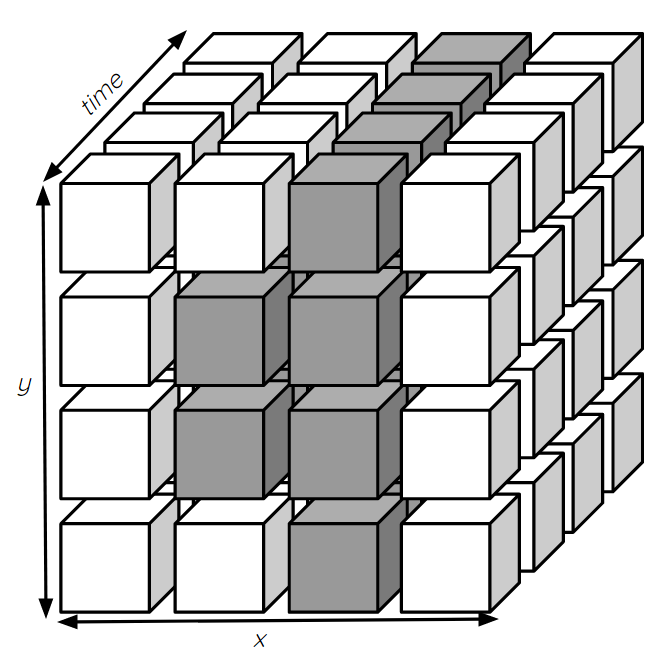
\includegraphics[width=0.4\linewidth]{image/general/atom_ROI.PNG} &  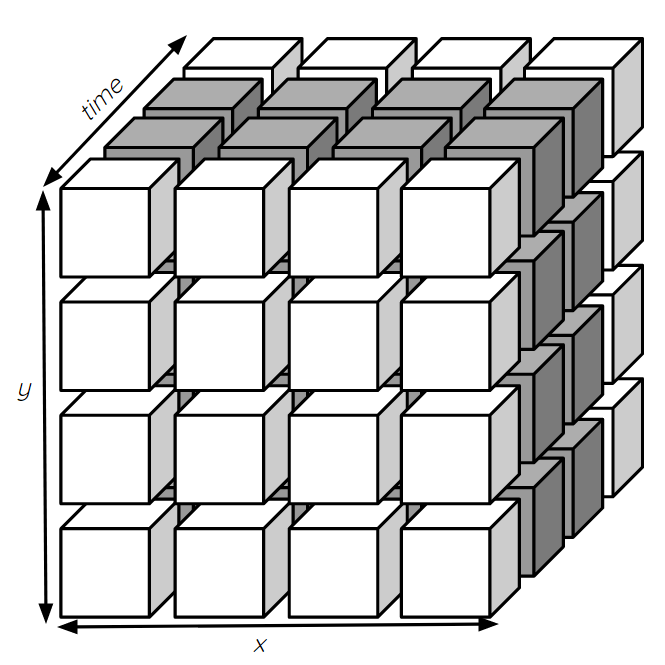
\includegraphics[width=0.4\linewidth]{image/general/atom_time_slicing.PNG}\\
(a) Region of Interest & (b) Time Slicing
\end{tabular}


\caption{Types of Queries} \label{fig:typesofQuery}
\end{figure}


\begin{comment}
\section{Database Schema}

\cc{do i need a database schema section?}

\end{comment}


\section{Semantic Extraction} 
\label{section:semanticsExtraction}

As object specific semantics from the scene provides deeper insights for surveillance purposes, as mention earlier, this work focuses on the extraction of two types of object specific semantics. These low level semantics are the Color and Motion semantics. Although several other semantics were extracted as well, the extraction of those semantics is not discussed in detail as they are simple extracting based on input data filenames. Table \ref{table:semantics} lists down all the semantics which were extracted in this work. The following subsections focuses on both the color and motion low-level semantics extraction process and framework.  



\begin{table} \centering
\caption {Types of Extracted Semantics and the Methods used}
\label{table:semantics}
\begin{tabular}{|l|l|l|}
\hline
\textbf{No.} & \textbf{Semantics Type} & \textbf{Method(s)}                                                                                                          \\ \hline
\textbf{1}   & Date                    & Filename data extraction                                                                                                         \\ \hline
\textbf{2}   & Time                    & Filename data extraction                                                                                                         \\ \hline
\textbf{3}   & Color                   & \begin{tabular}[c]{@{}l@{}}i) Handcrafted Feature \& Distance Estimation (HSV)\\ ii) Distance Estimation (Luv)\end{tabular} \\ \hline
\textbf{4}   & Motion                  & \begin{tabular}[c]{@{}l@{}}i) Handcrafted Feature\\ ii) Collection of Centroids\end{tabular}                                \\ \hline
\textbf{5}   & Object Type             & Deep Learning                                                                                                               \\ \hline
\textbf{6}   & Size                    & Bounding box from Background Subtraction                                                                                                      \\ \hline
\end{tabular}

\end{table}



\subsection{Color Semantic}
\label{subsec:colorsemantics}

Without a doubt, color information plays a significant role in field of useful semantics as it is often one of the most common information a user provides when they are tasked to describe an object from a given event in a particular scene. However, the process of extracting color information accurately is extremely challenging, especially in an outdoor setting. In these settings, the white balance of the said scene would appear very differently depending on various factors such as the ambient illumination during the different hours of the day or even weather conditions such as cloudy, rainy or sunshine would affect the overall scene. Several commercially available product such as 'Nix color sensor' \cite{nixsensorltd} and 'Adafruit RGB sensor' \cite{adafruit} makes use of an independent light source which has been calibrated as a means to tackle this challenge.

As color terms are commonly derived from the Munsell Color system which created in the early 20th century by Professor Albert H. Munsell, this color system was investigated further to examined how the color terms were defined for the color extraction process. The Munsell Color System was designed to organize colors the way the human's eye sees - which is, by organizing colors according to their hues, followed by the chromatic range and the brightness values in a perceptually uniform manner. For each horizontal circle, the hues can be divided into 5 principle hues which are Red, Yellow, Green, Blue, and Purple. This setup allows another 5 intermediate hues between each principle hues, for example: Green-Blue hue, Purple-Red hue. 

However, as previously discussed in Section \ref{section:litreview}, various color terms are used in the myriad of available standards. In the computing field, this creates a whole lot of problem as color terms are often presented with differing definitions and values. Hence, there is a dire need of determining the best way to extract and represent color values with its corresponding color terms. While the basic idea of colors seems to be a relatively simple idea for humans, machines on the other hand, do not understand the concept of colors. Modern computers generally represents color values using the Red-Green-Blue (RGB) values for most applications. Despite its frequent usage, it is difficult for humans to visualize a particular color when presented with three RGB values as these values does not directly translate the intuitive nature of a particular color. Along with that, it is also very difficult to visualize the difference between two colors using the RGB values only. 


\begin{figure}[htb!]
  \centering
\begin{tabular}{cc}
 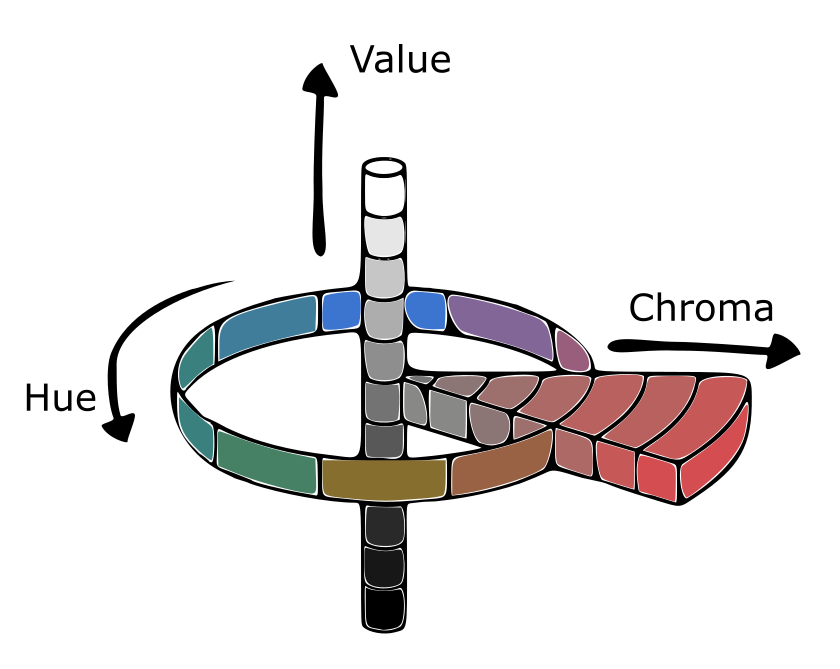
\includegraphics[width=0.4\linewidth]{image/general/munsell.png}  &
 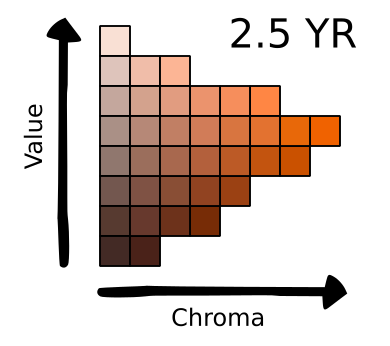
\includegraphics[width=0.4\linewidth]{image/general/25YR.png}\\
 (a) Munsell Color System &
(b) Hue at 2.5YR with various Chroma and Value\\
\end{tabular}
\caption{Munsell Color System} \label{fig:munsell}
\end{figure}


Figure \ref{fig:munsell}(b) illustrates the property of the chroma and value scale available on the Munsell color system, for example, a hue at 2.5 Yellow-Red (YR) has a maximum chroma value which differs along the value axis. While the Munsell Color system provided a significant contribution in color term naming research, the irregularity along the chroma and value axis does not translate well in a modern color space as the modern color spaces are uniformly distributed along all axis. Hence, in order to better represent the color space, this work chose to work primarily on the Hue-Saturation-Value (HSV) color space with some minor usage of other color spaces. The use of the HSV color space is twofold, firstly, the ease of color representation as it closely resembles the Munsell Color System, and secondly the distance between two colors are now intuitive and linear. As HSV color space is commonly used, the conversion between the RGB and HSV color spaces are seamless and can easily introduced into the existing processing framework. 

\begin{table}[]
\centering
\begin{tabular}{|c|c|c|}
\hline
\multicolumn{1}{|c|}{\textbf{Web Color Dictionary}} & \multicolumn{1}{c|}{\textbf{Number of Color Terms}} & \multicolumn{1}{c|}{\textbf{Year}} \\ \hline
x11 (R3)                                            & 631                                                 & 1988                               \\ \hline
HTML                                                & 140                                                 & Current                            \\ \hline
CSS                                                 & 148                                                 & Current                            \\ \hline
Crayola                                             & 248                                                 & Current                            \\ \hline
xkcd                                                & 954                                                 & 2010                               \\ \hline
\end{tabular}
\caption{Web Color Dictionary and the corresponding number of color terms}
\label{table:allcolorterms}
\end{table}




\begin{figure}[hbt!]\centering
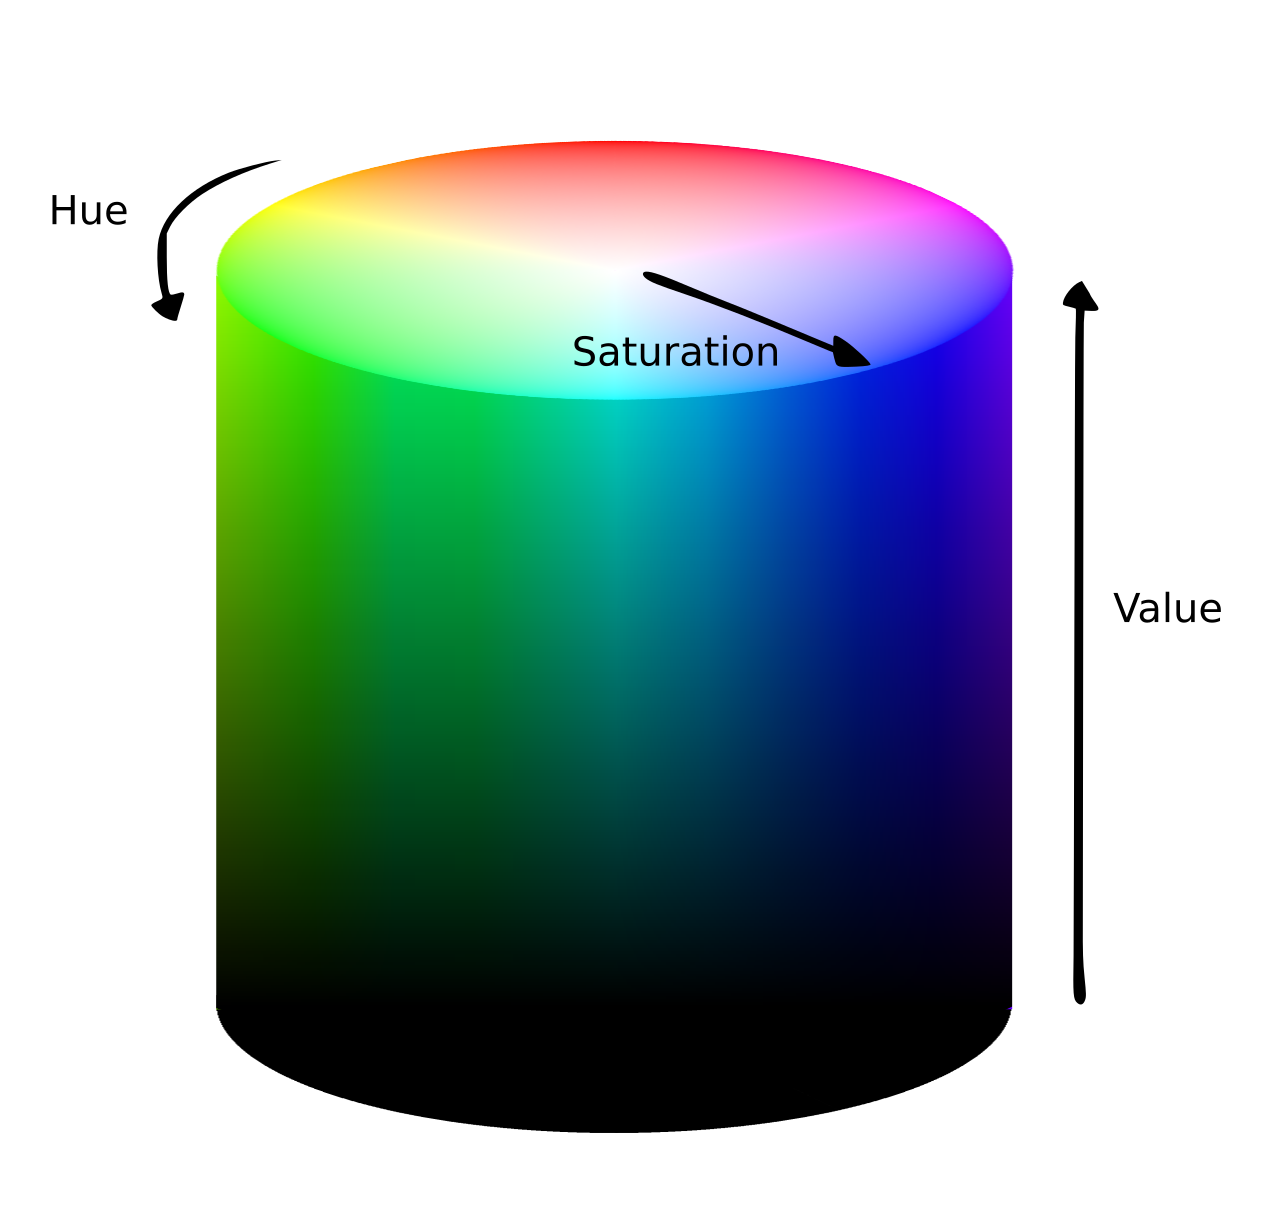
\includegraphics[width=.5\textwidth]{image/general/HSV.png}
\caption{Hue-Saturation-Value (HSV) Cylinder Visualization}
\label{fig:hsvcylinder}
\end{figure}


%https://people.csail.mit.edu/jaffer/Color/Dictionaries
% x11 colors: https://groups.google.com/forum/?fromgroups=#!topic/comp.windows.x/AYPozZhQxok
% https://www.crayola.com/explore-colors.aspx


Table \ref{table:allcolorterms} lists several famous web color dictionary along with the number of color categories available in each of those color standards. Given that there are so many different color categories, this ultimately leads to another set of question: "How many color categories should be extracted for the color semantic? And why?". In this work, the eleven basic color terms in English proposed in a classic study of worldwide color naming by \cite{berlinandkay} was adopted. In their study, Berlin and Kay proposed that the naming of colors terms may differ due to different cultures, based on their findings, native English language speakers generally used eleven basic color terms. These terms had to have three common properties which are: i) Highly used, ii) Monolexemic - meaning a single(mono) word, and not compounded color term such as 'baby blue', and iii) agreed upon by native speakers of the language. With those definitions, the common color terms proposed are black, white, gray, brown, red, orange, yellow, purple, green, blue, and pink. However, the definition of color terms by themselves are insufficient and invokes another set of challenge, which is the representation of these colors in numerical terms which are commonly used in computer science. 

However, those basic color terms defined were not associated with how colors are represented on a modern computer. Anatomically, there are three types of cons in the human retina, each of which are responsible over the receptiveness of colors in a particular type of wavelength. These wavelengths can be classified into three main categories: Short wavelengths light (420–440 nm), Medium  wavelengths light (534–545 nm) and Long wavelengths light (564–580 nm). As the number of con cells in the retina varies from each person, this, in turn affects the color perception of everyone. That, compounded with the fact that most monitor screens are not color calibrated professionally provided an opportunity for Munroe \cite{munroe2010color} to perform a internet wide crowd-sourcing survey on color terms and their respective numeral representation according to how colors are displayed on typical monitors.

In Munroe's experiments, 222,500 user sessions consisting of 40,000 women and 100,000 men, provided over five million colors their respective color terms. With the collected results, Munroe then proceeds to map a RGB tuple to a particular color term according to the highest frequency of responses. The mapping of these terms were done by averaging results of several stochastic hill climbing algorithms. At the end of Munroe's experiment, 954 color terms were assigned to a set of RGB tuples of equal size. Figure \ref{fig:xkcd} shows the mapping of dominant color terms over three fully saturated faces of the RGB cube. Now, by combining the work of Berlin and Kay along with the work of Munroe, the eleven basic color terms can now be translated into modern color tuples using the information collected. These color terms and the corresponding HEX values are listed in Table \ref{table:colorshex} and in this work, these values are treated as ground truth color data. 


\begin{figure}[hbt!]\centering
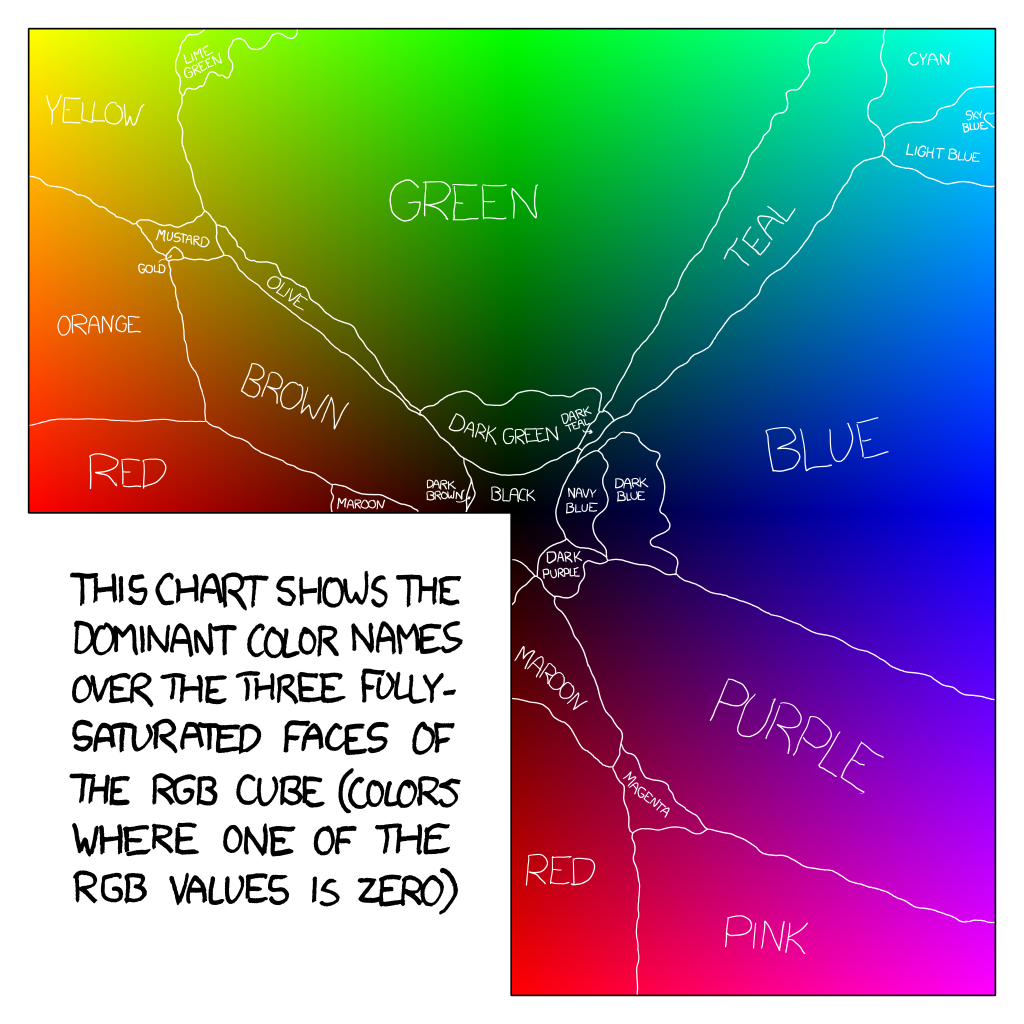
\includegraphics[width=.6\textwidth]{image/general/xkcd.png}
\caption{Dominant Color Terms over Three Fully Saturated Faces of the RGB Cube}
\label{fig:xkcd}
\end{figure}







% Please add the following required packages to your document preamble:
% \usepackage[table,xcdraw]{xcolor}
% If you use beamer only pass "xcolor=table" option, i.e. \documentclass[xcolor=table]{beamer}
\begin{table}[]\centering
\begin{tabular}{lcccc}
\cline{2-4}
\multicolumn{1}{l|}{}                     & \multicolumn{1}{l|}{\cellcolor[HTML]{000000}} & \multicolumn{1}{l|}{\cellcolor[HTML]{FFFFFF}} & \multicolumn{1}{l|}{\cellcolor[HTML]{929591}} &                                               \\ \cline{1-4}
\multicolumn{1}{|l|}{\textbf{HEX}}        & \multicolumn{1}{c|}{\#000000}                 & \multicolumn{1}{c|}{\#ffffff}                 & \multicolumn{1}{c|}{\#929591}                 &                                               \\ \cline{1-4}
\multicolumn{1}{|l|}{\textbf{Color Term}} & \multicolumn{1}{c|}{Black}                    & \multicolumn{1}{c|}{White}                    & \multicolumn{1}{c|}{Gray}                     &                                               \\ \cline{1-4}
                                          & \multicolumn{1}{l}{}                          & \multicolumn{1}{l}{}                          & \multicolumn{1}{l}{}                          &                                               \\ \cline{2-5} 
\multicolumn{1}{l|}{}                     & \multicolumn{1}{l|}{\cellcolor[HTML]{653700}} & \multicolumn{1}{l|}{\cellcolor[HTML]{E50000}} & \multicolumn{1}{l|}{\cellcolor[HTML]{F97306}} & \multicolumn{1}{l|}{\cellcolor[HTML]{FFFF14}} \\ \hline
\multicolumn{1}{|l|}{\textbf{HEX}}        & \multicolumn{1}{c|}{\#653700}                 & \multicolumn{1}{c|}{\#e50000}                 & \multicolumn{1}{c|}{\#f97306}                 & \multicolumn{1}{c|}{\#ffff14}                 \\ \hline
\multicolumn{1}{|l|}{\textbf{Color Term}} & \multicolumn{1}{c|}{Brown}                    & \multicolumn{1}{c|}{Red}                      & \multicolumn{1}{c|}{Orange}                   & \multicolumn{1}{c|}{Yellow}                   \\ \hline
                                          & \multicolumn{1}{l}{}                          & \multicolumn{1}{l}{}                          & \multicolumn{1}{l}{}                          &                                               \\ \cline{2-5} 
\multicolumn{1}{l|}{}                     & \multicolumn{1}{l|}{\cellcolor[HTML]{7E1E9C}} & \multicolumn{1}{l|}{\cellcolor[HTML]{15B01A}} & \multicolumn{1}{l|}{\cellcolor[HTML]{0343DF}} & \multicolumn{1}{l|}{\cellcolor[HTML]{FF81C0}} \\ \hline
\multicolumn{1}{|l|}{\textbf{HEX}}        & \multicolumn{1}{c|}{\#7e1e9c}                 & \multicolumn{1}{c|}{\#15b01a}                 & \multicolumn{1}{c|}{\#0343df}                 & \multicolumn{1}{c|}{\#ff81c0}                 \\ \hline
\multicolumn{1}{|l|}{\textbf{Color Term}}  & \multicolumn{1}{c|}{Purple}                   & \multicolumn{1}{c|}{Green}                    & \multicolumn{1}{c|}{Blue}                     & \multicolumn{1}{c|}{Pink}                     \\ \hline
\end{tabular}
\caption{Color Terms and the corresponding HEX value}
\label{table:colorshex}
\end{table}



\subsection{Motion Semantic}

The use of video data for surveillance purposes no doubt lies in its ability to capture motion information. These information are usually provided by users when tasked to describe an action which occurred in a given scene. In this work, the collection motion performed by a vehicle in the scene is denoted as a vehicle's trajectory.  

Typically, a user describes motion information using a combination of several information such as time of occurrence, location and how the motion occurred. Traditionally, the motion information from videos are converted into text based descriptions using handcrafted methods. Given the following example: "A yellow vehicle was turning into the cross section between Road Alpha and Road Beta at 3:30pm when a black vehicle came rushing over and hitting a pedestrian in the process during commotion", this statement could be converted into a statement such as "yellow car turn left Road Alpha and Road Beta". 

While motions are not as subjective as the concept of colors, text based descriptions of motion events are less intuitive when compared to a graphical description. Hence, this work aims to extract motion information and present them in a graphical form which is naturally more intuitive hence providing an accurate description of an event.



In the case of a carpark scene, the trajectory information from each vehicle is important, it is a paramount task to ensure that the motion information from each vehicle is captured and stored. Since the types of motion performed in a carpark setting varies from user to user, instead of generating a fine representation of motion such the conventional motion vector, these information were broken into smaller motion information and stored into the database. Both the suggested motion semantics extraction frameworks deploys different extraction methods which would be discussed further in this chapter.




%In the following subsections, the details of both implementations of semantic extraction frameworks are discussed in detail. 


\subsection{Other Semantic}

In this subsection, the extraction process of the other low level semantics are discussed briefly. As mentioned earlier, several other semantics were extracted for this work, namely, the time and date information, object type as well as object size. As the extractions of these semantics were simple and/or played little-to-no roles in the both the extraction module and retrieval engine, the process will be described here.

\subsubsection{Date \& Time}
During course of the dataset collection, the camera was set to name the recorded files according to the time and date. As described in Section \ref{section:dataset_used}, the camera was set to record video clips from 8:30am to 6:30pm in the evening with each clip being 6 minutes long. As the filename contains both the time and date information, the date information can be easily extracted while the time information can be deduced when a vehicle is observed in the carpark scene. 

\begin{align}
\label{eq:file_timing}
	Current Frame Time = (Video Duration [6 mins] \times \frac{Current Frame}{Total Frames}) + Time_{filename} 
\end{align}


Upon extracting these information, simple formating is done to ensure these information conform to the typical SQL database requirements.

\subsubsection{Object Type \& Size}
Since the object of interest in this work are the vehicles in the carpark scene, YOLOv2 was used to assist the validation of the foreground object detected by the background subtraction method as described in Section \ref{subsection:fundamental}. With that in place, all the objects which were detected were assumed to fall under the "vehicle" class. As for the object size, the foreground objects' bounding box's size were saved in the database as the object size.





\section{\versionOne }
\label{section:semantic_lsh}

\subsection{Overview}
Before diving deeper into the nitty-gritty of the \versionOne, first, the term Locality Sensitive Hashing needs to be addressed. LSH is a technique used for its ability in dimensionality reduction, this technique excels especially when working with high dimensional data such video data. 

This is done by hashing documents with similar properties, mapping and clustering them into a similar neighbourhood. Hence, reducing the dimensionality of a large document in the process. However, since the exact implementation of LSH is not used in this work, the focus will be anchored on the idea of clustering documents with similar properties in the same neighbourhood. 


\begin{figure}[hbt!]\centering
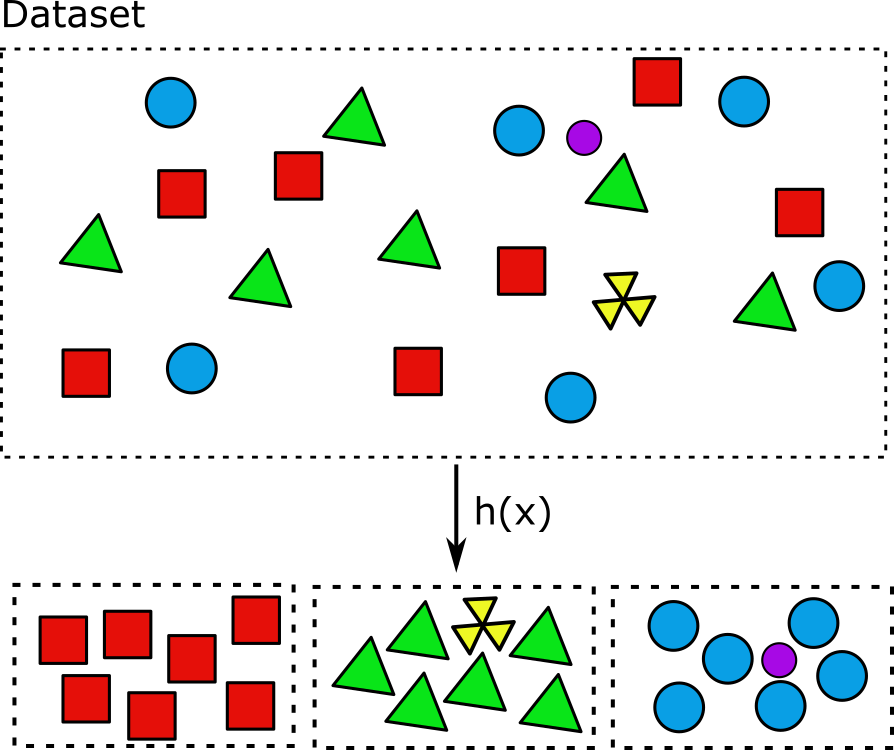
\includegraphics[width=.7\textwidth]{image/lsh.png}
\caption{Locality Sensitive Hashing}
\label{fig:lshexample}
\end{figure}

In the \versionOne, each extracted semantic property is defined as a document. A total of 11 color semantic clusters as well as 9 motion semantic clusters were assigned. In this implementation, each cluster was represented using an SQL table. During the semantic extraction process, documents with similar properties were inserted into the same table as the clustering method. 


\subsection{Color Semantic Extraction }
%With that in place, this setting effectively performs quantize the range of colors to a fixed number of color categories while taking advantage of the atom-based structure (Refer to Section \ref{SemanticSegmentation}).

As the background subtraction module has separated the foreground blobs from background scene, these blobs are now assigned a bounding box using the blob's maximum and minimum value on both axis. These bounding box are used to mark the location of the vehicle when a vehicle is detected in the scene. However, due to the background subtraction method used, the final foreground blob tend to appear somewhat larger than the actual vehicle footprint. 

In order to minimize noise from the bounding box and to obtain a closer estimation of the vehicle's dominant color, the bounding box is cropped by a factor of 30\% to reduce background noise such as the tar road or vehicles close to it. In order to maintain as much information, the bounding box was not reduced further as that often results in the cropping of the vehicle's windscreen and window regions, thus altering the overall dominant color.

Now that the bounding box has been cropped, the next strategy was implemented to determine the dominant color of each vehicle by first distinguishing between chromatic and achromatic vehicles. Following similar definition of achromatic colors from Munsell, achromatic colors also known as neutral colors are characterized by the lack of strong hue or chroma values such as black, white and gray color. This process starts off by comparing the cropped image against a grayscale version of the same image. Next, the obtained absolute difference between these images were subjected to a threshold process for all three channels in the RGB color space. The step was done to effectively amplify the difference between the original image and the grayscale image, pixels with values above the threshold value were set to the maximum value of 255. The threshold value used for this step was empirically set at 35. Finally, the output of the process was converted to the grayscale color space. The hint of significant values at this stage provided an indication of substantial presence of chromatic hues for this particular vehicle.     

With the interest of differentiating between chromatic and achromatic vehicles, the ratio of non-zero pixel value over the total pixels in an image were obtained. This threshold pivot value, $T_{pivot}$, was empirically set at 18\% where vehicles blobs that exceeds this value were assumed to contain strong chromatic hue. The entire process from the original image to the deduction of whether a vehicle blob was chromatic or achromatic is illustrated using Figure \ref{fig:achromatic_thresh}. This handcrafted algorithm allows the deduction of strong chromatic hues and estimates if a particular vehicle blob belongs to a chromatic or achromatic subset. 


\begin{figure}[htb!]
  \centering
\begin{tabular}{c}
 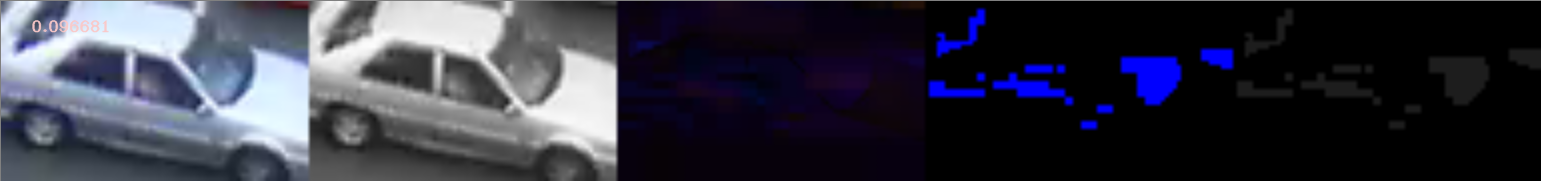
\includegraphics[width=0.9\linewidth]{image/general/achromatic_threshold5.PNG} \\  
 (a) Achromatic vehicle (Gray/White) \\
 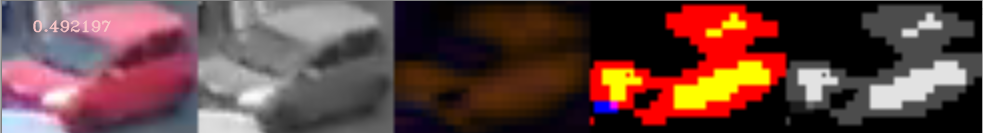
\includegraphics[width=0.9\linewidth]{image/general/achromatic_threshold_color2.PNG}\\
(b) Chromatic vehicle (Red)
\end{tabular}
\caption{(From left) Original image; Grayscale image; Absolute difference; Binary threshold absolute difference; Threshold difference in grayscale} \label{fig:achromatic_thresh}
\end{figure}



\paragraph{Achromatic and chromatic color processing.} Upon determining whether or not the vehicle belongs to the achromatic scale using the $T_{pivot}$ value, the cropped images were then subjected to both the black and white color filters individually. These simple filters were designed using binary thresholds values empirically set at an intensity levels of 50 and 170 respectively. Next, using a similar fashion, the ratio of non-zero pixels upon filtering were computed. These non-zero percentage ration was used to determine if the vehicle belongs to black, white or gray color terms. Figure \ref{fig:blackwhite_filter} shows how a white vehicle responds to a black and white filter. 

\begin{figure}[hbt!]\centering
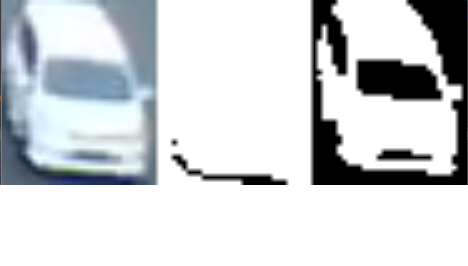
\includegraphics[width=.7\textwidth]{image/general/blackwhitefilter.PNG}
\caption{Black \& While Filter Response of a White Vehicle}
\label{fig:blackwhite_filter}
\end{figure}


 \begin{algorithm}[!ht]
  \caption{Achromatic Color}
  \label{algo:achromatic}
  \begin{algorithmic}[1]
  
  \If{Percentage of White $>$ 25\%  \\
  \hspace{1em} \&\& Percentage of Black $<$ 25\%}
	\State Color Term = White  	
  \ElsIf {Percentage of Black $>$ 25\%  \\ 
  \hspace{1em} \&\& Percentage of White $<$ 25\%}
  	\State Color Term = Black
  \Else
  	\State Color Term = Gray
  \EndIf
  
  \end{algorithmic}
\end{algorithm}

 
 \begin{algorithm}[!h]
  \caption{Color Term Extraction}
  \label{algo:colorExtract}
  \begin{algorithmic}[1]
    \For{Each blob in object}
        \State Shrink bounding box \& crop image
        \State Create a copy of the cropped image in grayscale
        \State Compute absolute difference between cropped image \& grayscale image
        \State Perform threshold on absolute difference to amplify difference
        \State Convert results into grayscale \& calculate no. of non-zero pixels
            \If{Ratio of non-zero pixels $>$ $T_{pivot}$} 
                \State // Chromatic Vehicle
                \State Calculate 3D HSV histogram  
                \State Locate maximum bin location of each channel
                \State Map the highest bin from each channel to Color Term
            \Else 
                \State // Achromatic Vehicle
                \State Perform black \& white filter 
                \State Obtain ratio of non-zero pixels from both filters
                \State Determine Color Term
            \EndIf

    \EndFor
    \State Obtain average dominant color \& return Color Term
  \end{algorithmic}
\end{algorithm}


As previously mention, this work chose to primarily work on the HSV color space, this applies especially for the chromatic color extraction process. First, the cropped image was converted to the HSV color space. Then, a 3-Dimensional histogram of the cropped image was generated to identify the maximum value of each channel. However, as colors belongs to a spectrum, using a fine-grained histogram is not ideal as the generated output would be spread across a segment. Hence, the HSV channels were quantized into the following settings: 15 Hue bins, 8 Saturation bins and 8 Value bins for the histogram generation. 






% Please add the following required packages to your document preamble:
% \usepackage[table,xcdraw]{xcolor}
% If you use beamer only pass "xcolor=table" option, i.e. \documentclass[xcolor=table]{beamer}
\begin{table}[]\centering
\resizebox{\textwidth}{!}{
\begin{tabular}{c|c|c|c|c|c|c|c|c|c|c|c|}
\cline{2-12}
\multicolumn{1}{l|}{}                        & \multicolumn{11}{c|}{\textbf{Similarity(\%) Based on $D_{Euclidean}$ in HSV Color Space}}                                                                                                                                                                                       \\ \hline
\multicolumn{1}{|c|}{\textbf{Bin/Color}} & \textbf{Black} & \textbf{Blue} & \textbf{Brown} & \textbf{Gray}                          & \textbf{Green}                         & \textbf{Orange} & \textbf{Pink}                          & \textbf{Purple}                        & \textbf{Red} & \textbf{White} & \textbf{Yellow} \\ \hline
\multicolumn{1}{|c|}{ 
\begin{tabular}{c}  \\

\includegraphics[width=0.1\linewidth]{image/HSVcolorspace/img_0_4_7.jpg} \\  
\textbf{0, 4, 7} 
\end{tabular}     }  

& 30.46          & 67.06         & 55.74          & 57.51                                  & 70.94                                  & 73.76           & \cellcolor[HTML]{9AFF99}\textbf{92.18} & 71.95                                  & 72.25        & 64.00          & 76.33           \\ \hline
  
\multicolumn{1}{|c|}{ 
\begin{tabular}{c}  \\

\includegraphics[width=0.1\linewidth]{image/HSVcolorspace/img_2_4_3.jpg} \\  
\textbf{2, 4, 3} 
\end{tabular}     }  


& 54.07          & 60.33         & 70.03          & 59.16                                  & 66.14                                  & 55.81           & 64.00                                  & \cellcolor[HTML]{9AFF99}\textbf{81.03} & 59.25        & 49.04          & 55.33           \\ \hline

\multicolumn{1}{|c|}{ 
\begin{tabular}{c}  \\

\includegraphics[width=0.1\linewidth]{image/HSVcolorspace/img_3_7_4.jpg} \\  
\textbf{3, 7, 4} 
\end{tabular}     }  

& 29.70          & 73.77         & 86.97          & 42.04                                  & \cellcolor[HTML]{9AFF99}\textbf{90.03} & 72.85           & 58.01                                  & 78.43                                  & 76.15        & 33.49          & 72.24           \\ \hline
\multicolumn{1}{|c|}{ 
\begin{tabular}{c}  \\

\includegraphics[width=0.1\linewidth]{image/HSVcolorspace/img_6_2_6.jpg} \\  
\textbf{6, 2, 6} 
\end{tabular}     }  


& 41.35          & 56.33         & 46.77          & \cellcolor[HTML]{9AFF99}\textbf{75.87} & 62.87                                  & 53.88           & 72.91                                  & 62.49                                  & 52.12        & 69.89          & 58.04           \\ \hline



% ----- remove these? 

\multicolumn{1}{|c|}{ 
\begin{tabular}{c}  \\

\includegraphics[width=0.1\linewidth]{image/HSVcolorspace/img_11_0_0.jpg} \\  
\textbf{11, 0, 0} 
\end{tabular}     } &  

\cellcolor[HTML]{9AFF99}\textbf{88.15} &	21.74 &	35.36 &	60.73 &	31.88 &	17.02 &	34.30 &	41.36 &	19.80 &	39.59 &	17.52
\\ \hline

\multicolumn{1}{|c|}{ 
\begin{tabular}{c}  \\

\includegraphics[width=0.1\linewidth]{image/HSVcolorspace/img_11_0_1.jpg} \\  
\textbf{11, 0, 1} 
\end{tabular}     }  &
\cellcolor[HTML]{9AFF99}\textbf{83.66} &	26.71 &	37.51 &	67.13 &	36.19 &	22.35 &	41.39 &	45.70 &	24.80 &	47.38 &	23.04
\\ \hline

\multicolumn{1}{|c|}{ 
\begin{tabular}{c}  \\

\includegraphics[width=0.1\linewidth]{image/HSVcolorspace/img_11_0_2.jpg} \\  
\textbf{11, 0, 2} 
\end{tabular}     }  &
\cellcolor[HTML]{9AFF99}\textbf{77.20} &	31.13 &	38.69 &	72.71 &	39.75 &	27.21 &	48.22 &	49.15 &	29.27 &	55.12 &	28.11
\\ \hline

\multicolumn{1}{|c|}{ 
\begin{tabular}{c}  \\

\includegraphics[width=0.1\linewidth]{image/HSVcolorspace/img_11_0_3.jpg} \\  
\textbf{11, 0, 3} 
\end{tabular}     }  & 
70.02 &	34.87 &	38.85 &	\cellcolor[HTML]{9AFF99}\textbf{76.86} &	42.43 &	31.48 &	54.68 &	51.54 &	33.08 &	62.76 &	32.61     
\\ \hline

\multicolumn{1}{|c|}{ 
\begin{tabular}{c}  \\

\includegraphics[width=0.1\linewidth]{image/HSVcolorspace/img_11_0_4.jpg} \\  
\textbf{11, 0, 4} 
\end{tabular}     }  &
62.53 &	37.82 &	37.98 &	\cellcolor[HTML]{9AFF99}\textbf{78.73} &	44.10 &	35.06 &	60.60 &	52.69 &	36.13 &	70.25 &	36.44 
\\ \hline

\multicolumn{1}{|c|}{ 
\begin{tabular}{c}  \\

\includegraphics[width=0.1\linewidth]{image/HSVcolorspace/img_11_0_5.jpg} \\  
\textbf{11, 0, 5} 
\end{tabular}     }  &
54.88 &	39.85 &	36.13 &	\cellcolor[HTML]{9AFF99}\textbf{77.73} &	44.67 &	37.83 &	65.69 &	52.53 &	38.30 &	77.42 &	39.47
\\ \hline

\multicolumn{1}{|c|}{ 
\begin{tabular}{c}  \\

\includegraphics[width=0.1\linewidth]{image/HSVcolorspace/img_11_0_6.jpg} \\  
\textbf{11, 0, 6} 
\end{tabular}     }  &
47.14 &	40.88 &	33.38 &	74.20 &	44.10 &	39.67 &	69.54 &	51.05 &	39.50 &	\cellcolor[HTML]{9AFF99}\textbf{83.84} &	41.56    
\\ \hline

\multicolumn{1}{|c|}{ 
\begin{tabular}{c}  \\

\includegraphics[width=0.1\linewidth]{image/HSVcolorspace/img_11_0_7.jpg} \\  
\textbf{11, 0, 7} 
\end{tabular}     }  &
39.35 &	40.84 &	29.83 &	68.98 &	42.43 &	40.49 &	71.62 &	48.38 &	39.665 &	\cellcolor[HTML]{9AFF99}\textbf{88.23} &	42.61      
\\ \hline



% ----- remove these? 


\end{tabular}}
\caption{Samples of Similarity Score(\%) based on Euclidean Distance in HSV Color Space, Highlighted in Green is the Highest Scoring Color Term}
\label{tab:hsvExample}
\end{table}










This setup ends up with a total of 960 bins where each of these bins are assigned a single color term based on the closest euclidean distance between this bin's color and the highest scoring ground truth color term using the HSV color space. Using this setup, the color term which corresponds to the bin(h,s,v) which contains the highest number of hits for a given image is assigned. The examples in Table \ref{tab:hsvExample} shows samples of bins and their corresponding similarity score. However, since the vehicles are moving in the outdoor setting, the ambient and directional lighting (from sun and other light sources) contribute to slight variation of colors. To accommodate the varying lighting condition, the dominant color of each tracked vehicle from each frame was averaged out throughout its trajectory as illustrated in \ref{fig:ADC}. 


As the entire process was done repeatedly over every single frame in the video, the color term of a particular vehicle is saved into the database while it is tracked. As such, a single vehicle could be classified as a variety of colors depending on the location on where the vehicle was tracked. Algorithm \ref{algo:colorExtract} summarizes the strategy used for color semantic extraction process for the \versionOne. 



\subsection{Motion Semantic Extraction}


In order to extract motion information of vehicles, the initial step of obtaining the foreground objects from the background subtraction method still stands. Upon identifying these foreground objects, the locations of each vehicles are obtained using the centroids using Equation \ref{eq:centroid}. The motions were extracted by naive position displacement inference methods. Next, the centroids of the vehicles from each frame ($P_N$) are stored in a list, \H{L}. 

As two subsequent frames is likely to have too little difference, the algorithm was set to wait until the list has at least 10 records of the previous position before extracting the motion information. Algorithm \ref{algo:motion} provides details of this semantic extraction process in pseudo-code. In this work, the motion of a vehicle is quantized into 8 directional bins (in the form of four cardinal directional and four intermediate directional bins) along with another bin which denotes minuscule and negligible motion information. These quantized directions can be categorized into: UP, DOWN, LEFT, RIGHT, LEFT-UP, LEFT-DOWN, RIGHT-UP, RIGHT-DOWN, MOTIONLESS. 

Figure \ref{fig:cardinalbins} illustrates this property. Each of this directions are determined using handcrafted parameters which were selected empirically, the displacement values, $X_{displacement}$ \& $Y_{displacement}$ were set to 5 pixels each. If the difference between the current position of the blob and the position 10 frames ago is larger than either $X_{displacement}$ or $Y_{displacement}$, the motion of the vehicle is updated accordingly. The extracted motion semantic is then saved into the database for each frame. 


 \begin{algorithm}[!h]
	\caption{Motion Semantic Extraction}
	\label{algo:motion}
	\begin{algorithmic}[1]
		\For{Each blob}
		\State Save current centroid position$P_N$ in $List_{motion}$, \H{L} 
		\If{\H{L}.length > 10} 
		\State Calculate $Difference_x$ and $Difference_y$ using:
		\State $Difference_{centroid} = P_N -P_{(N-10)}$
		\If {Absolute ($Difference_{x}$) > $X_{displacement}$ }
		\If {$Difference_{x}$ > 0 }
		\State Set \textit{Direction(X)} to "LEFT"
		\Else 
		\State Set \textit{Direction(X)} to "RIGHT"
		\EndIf
		\EndIf
		\If {Absolute ($Difference_{y}$) > $Y_{displacement}$ }
		\If {$Difference_{y}$ > 0 }
		\State Set \textit{Direction(Y)} to "UP"
		\Else 
		\State Set \textit{Direction(Y)} to "DOWN"
		\EndIf
		\EndIf

		\If {\textit{Direction(Y)} != NULL AND \textit{Direction(X)} != NULL }
		\State Set blob's motion = \textit{Direction(X)} + \textit{Direction(Y)}
		\Else 
		\If {\textit{Direction(X)} != NULL }
		\State Set blob's motion = \textit{Direction(X) }
		\ElsIf  {\textit{Direction(Y)} != NULL }
		\State Set blob's motion = \textit{Direction(Y)}
		\Else 
		\State Set blob's motion = "Motionless"
		\EndIf
		\EndIf
		\EndIf
		\State Save blob's current motion into database
		\EndFor
	\end{algorithmic}
\end{algorithm}

\begin{figure}[hbt!]\centering
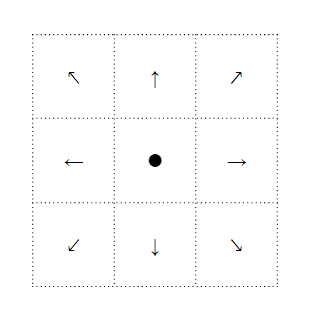
\includegraphics[width=.5\textwidth]{image/motion.PNG}
\caption{Directional bins setup}
\label{fig:cardinalbins}
\end{figure}





\section{\versionTwo }
\label{section:semantic_chamfer}


\subsection{Overview}

During the course of experimenting with the \versionOne, one of the drawbacks identified was that the semantic extraction process was too handcrafted. Although the results could have improved with more tweaking of the parameters and various knobs available, the process of experimenting what works best would be extremely tedious and the end product would not necessarily be extendable to other frameworks depending on the input data.

Along with that, there were several key issues which were identified that could be improved upon. One of the issue pinpointed was that the process of determining whether or not a vehicle belonged to achromatic or chromatic scale was biased. In the dataset on which the experiments were conducted on, there were a lot more achromatic vehicle compared to chromatic vehicle. As the scale was bias, it was easy to manipulate the overall retrieval results by adjusting the parameters to favor the achromatic scale. 

The aim of the \versionTwo is to provide alternative solutions and improve the performance of the \versionOne. In the following subsections, the color semantic extraction and motion semantic extraction is discussed in detail.

\subsection{Color Semantic Extraction}

As previously discussed in the section \ref{subsec:colorsemantics}, the basic idea of colors is relatively simple for humans, machines on the other hand, have a hard time understanding the concept of colors. In order to extract color semantics, the initial steps to obtain the Average Dominant Color (ADC) was inherited from the previous method where the bounding box of the detected vehicles from the background subtraction method were cropped. 

Next, the dominant color from each frame was extracted using the maximum bin of the 3-dimension HSV histogram and concatenated. At the end of a vehicle's tracked life cycle, the concatenated dominant colors were averaged out to obtain the ADC. The example in Figure \ref{fig:ADC} illustrates this method while the pseudo-code of the ADC method is described in Algorithm \ref{algo:ADC}.  


\begin{figure}[hbt!]\centering
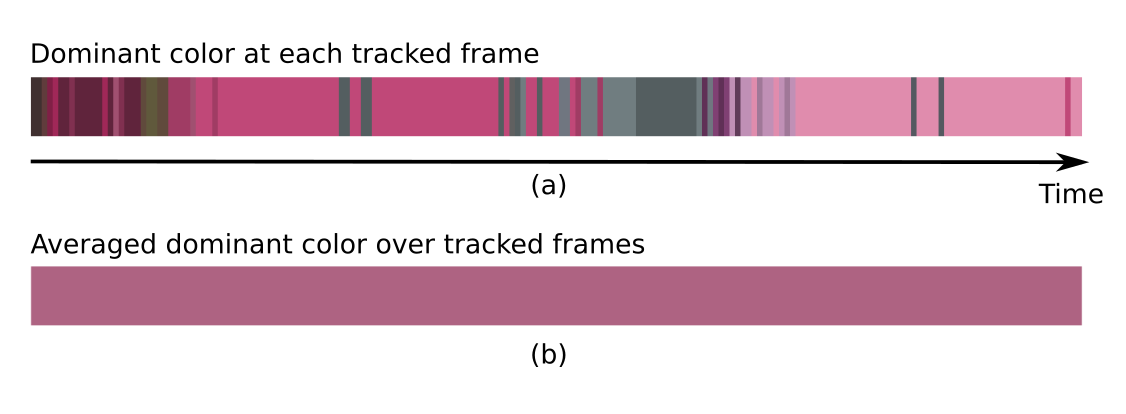
\includegraphics[width=.9\textwidth]{image/general/ADC.png}
\caption{(a) Dominant color of the vehicle at each frame; (b) Average dominant color}
\label{fig:ADC}
\end{figure}




\begin{algorithm}[!h]
  \caption{Average Dominant Color \& Similarity Score Determination}
  \label{algo:ADC}
  \begin{algorithmic}[1]
    \For{Each tracked vehicle in the current frame}
        \State Shrink bounding box (crop image)
        \State Calculate 3D HSV histogram
        \State Locate maximum bin location of each channel from histogram
        \State Concatenate resulting dominant colors from each frame
        \State Obtain the Average Dominant Color (ADC)
        \State Measure the difference between ground truth value from Munroe \cite{munroe2010color} 
        \State Obtain Similarity Score of color tuple against color terms
    \EndFor
  \end{algorithmic}
\end{algorithm}





In order to reduce the number of parameters and steer clear of handcrafted features such as the one introduced in the previous subsections, instead of assigning one single color term for each extracted, the similarity score for each color against all eleven ground truth colors were measured and saved into the database instead. The metrics used to measure the similarity scores between the colors were adopted from the work of Riemersma\cite{riemersma}. This metrics is a low cost estimation of the differences of colors in the LUV linear color space using RGB values. As the Average Dominant Color was obtained in the HSV color space, a quick conversion from HSV to RGB color space was done using Equation \ref{eq:RGBHSVconversion1} to \ref{eq:RGBHSVconversion3}. 


%% ---- RGBHSVconversion metric ------------------------------------------------
\begin{equation}
\label{eq:RGBHSVconversion1}
V = \max(R,G,B) 
\end{equation}

\begin{equation}
\label{eq:RGBHSVconversion2}
S = \begin{cases}\frac{V - \min(R,G,B)}{V} & , V \neq 0\\ 
0 & , otherwise \end{cases} \\
\end{equation}

\begin{equation}
\label{eq:RGBHSVconversion3}
H = \begin{cases}
\hspace{2.8em} \frac{60(G-B)}{V-\min(R,G,B)} & ,V = R\\
120 + \frac{60(B-R)}{V-\min(R,G,B)} & ,V = G\\
240 + \frac{60(R-G)}{V-\min(R,G,B)} & ,V = B 
\end{cases}
\end{equation}

\centerline{\\$\textit{if } \hspace{.8em}H< 0 \hspace{.8em}\textit{ then } \hspace{.8em}H = H+360.$}





%% ---- RGBHSVconversion metric ------------------------------------------------






According to Riemersma, the benefit of this metrics is that it is a far more stable algorithm where, as quoted, "it does not have a range of colours where it suddenly gives far from optimal results". First, the mean of both the Average Dominant Color(ADC) and Ground Truth Color (GTC)'s red channel were obtained. Then, this is followed by obtaining the difference, $\Delta$, of all three R, G, and B channels were obtained as well. 

In Equation \ref{eq:DiffColorLUV}, the mean of the red channel ($\mean{r}$) is used as a weight for both $\Delta{R}$ and $\Delta{B}$. The details of these equations is described in Equation \ref{eq:RedMeanRGBDiff} and \ref{eq:DiffColorLUV} respectively. Table \ref{tab:luvExample} uses the same example colors as used in Table \ref{tab:hsvExample}, however, the similarity score of the colors were calculated using the metric suggested in Equation \ref{eq:DiffColorLUV} instead of the Euclidean Distance measured in HSV color space.


%% ---- First metric ------------------------------------------------
\begin{equation}
\begin{split}
\label{eq:RedMeanRGBDiff}
\mean{r} = \frac{C_{1R} + C_{2R}}{2}
\end{split}
% \end{equation}
\quad\quad\quad ; \quad\quad\quad
% \begin{equation}
 \begin{split}
\Delta R = C_{1R} - C_{2R}\\ 
\Delta G = C_{1G} - C_{2G}\\ 
\Delta B = C_{1B} - C_{2B}
 \end{split}
\end{equation}

\begin{equation}
\label{eq:DiffColorLUV}
\Delta Color_{LUV} = \sqrt{(2 + \frac{\mean{r}}{256}) \times \Delta R^{2} + 4 \times \Delta G^{2} + (2 + \frac{255 - \mean{r}}{256}) \times \Delta B^{2} }
\end{equation}




%% ---- First metric ------------------------------------------------



% Please add the following required packages to your document preamble:
% \usepackage[table,xcdraw]{xcolor}
% If you use beamer only pass "xcolor=table" option, i.e. \documentclass[xcolor=table]{beamer}
\begin{table}[]\centering
\resizebox{\textwidth}{!}{
\begin{tabular}{c|c|c|c|c|c|c|c|c|c|c|c|}
\cline{2-12}
\multicolumn{1}{l|}{}                        & \multicolumn{11}{c|}{\textbf{Similarity(\%) Based on Riemersma's low cost LUV estimation metrics}}                                                                                                                                                                                       \\ \hline
\multicolumn{1}{|c|}{\textbf{Bin/Color}} & \textbf{Black} & \textbf{Blue} & \textbf{Brown} & \textbf{Gray}                          & \textbf{Green}                         & \textbf{Orange} & \textbf{Pink}                          & \textbf{Purple}                        & \textbf{Red} & \textbf{White} & \textbf{Yellow} \\ \hline
\multicolumn{1}{|c|}{ 
\begin{tabular}{c}  \\

\includegraphics[width=0.1\linewidth]{image/HSVcolorspace/img_0_4_7.jpg} \\  
\textbf{0, 4, 7} 
\end{tabular}     }  

& 
0.00 & 	0.91 & 	28.25 & 	61.27 & 	14.33 & 	67.17 & 	\cellcolor[HTML]{9AFF99}\textbf{70.97} & 	34.74 & 	31.11 & 	25.76 & 	37.78

\\ \hline
  
\multicolumn{1}{|c|}{ 
\begin{tabular}{c}  \\

\includegraphics[width=0.1\linewidth]{image/HSVcolorspace/img_2_4_3.jpg} \\  
\textbf{2, 4, 3} 
\end{tabular}     }  


& 
34.11 &	22.06 &	\cellcolor[HTML]{9AFF99}\textbf{68.39} &	59.91 &	56.72 &	46.89 &	27.22 &	46.24 &	31.23 &	0.00 &	15.51
\\ \hline

\multicolumn{1}{|c|}{ 
\begin{tabular}{c}  \\

\includegraphics[width=0.1\linewidth]{image/HSVcolorspace/img_3_7_4.jpg} \\  
\textbf{3, 7, 4} 
\end{tabular}     }  

& 
28.13 &	6.53 &	59.41 &	46.70&	\cellcolor[HTML]{9AFF99}\textbf{71.77} &	39.83 &	11.63 &	24.39 &	17.20 &	0.00 &	20.80
\\ \hline
\multicolumn{1}{|c|}{ 
\begin{tabular}{c}  \\

\includegraphics[width=0.1\linewidth]{image/HSVcolorspace/img_6_2_6.jpg} \\  
\textbf{6, 2, 6} 
\end{tabular}     }  


& 
0.00 &	18.72 &	3.55 &	\cellcolor[HTML]{9AFF99}\textbf{70.23} &	27.07 &	16.88 &	44.52 &	18.63 &	0.00 &	46.66 &	27.72
\\ \hline



% ----- remove these? 

\multicolumn{1}{|c|}{ 
\begin{tabular}{c}  \\

\includegraphics[width=0.1\linewidth]{image/HSVcolorspace/img_11_0_0.jpg} \\  
\textbf{11, 0, 0} 
\end{tabular}     } &  

\cellcolor[HTML]{9AFF99}\textbf{89.43}&  	15.88 & 	65.51 & 	10.69 & 	26.97 & 	4.79 & 	0.00& 	35.26 & 	23.58 & 	0.00 & 	0.00
\\ \hline

\multicolumn{1}{|c|}{ 
\begin{tabular}{c}  \\

\includegraphics[width=0.1\linewidth]{image/HSVcolorspace/img_11_0_1.jpg} \\  
\textbf{11, 0, 1} 
\end{tabular}     }  &
68.45 &	30.30 &	\cellcolor[HTML]{9AFF99}\textbf{73.87} &	31.62 &	39.47 &	18.66 &	1.26 &	51.17 &	29.17 &	0.00 &	0.00
\\ \hline

\multicolumn{1}{|c|}{ 
\begin{tabular}{c}  \\

\includegraphics[width=0.1\linewidth]{image/HSVcolorspace/img_11_0_2.jpg} \\  
\textbf{11, 0, 2} 
\end{tabular}     }  &
47.48 &	39.90 &	\cellcolor[HTML]{9AFF99}\textbf{68.14} &	52.51 &	46.37 &	29.69 &	20.24 &	61.69 &	29.45 &	0.00 &	0.00 
\\ \hline

\multicolumn{1}{|c|}{ 
\begin{tabular}{c}  \\

\includegraphics[width=0.1\linewidth]{image/HSVcolorspace/img_11_0_3.jpg} \\  
\textbf{11, 0, 3} 
\end{tabular}     }  & 
26.52& 	42.30& 	53.27& 	\cellcolor[HTML]{9AFF99}\textbf{73.32}& 	45.52& 	36.31& 	38.11& 	62.02& 	24.32& 	0.14& 	7.44
\\ \hline

\multicolumn{1}{|c|}{ 
\begin{tabular}{c}  \\

\includegraphics[width=0.1\linewidth]{image/HSVcolorspace/img_11_0_4.jpg} \\  
\textbf{11, 0, 4} 
\end{tabular}     }  &

5.57 &	36.68 &	35.26 &	\cellcolor[HTML]{9AFF99}\textbf{93.29} &	37.23 &	37.17 &	53.65 &	51.99 &	14.78 &	21.02 &	18.85

\\ \hline

\multicolumn{1}{|c|}{ 
\begin{tabular}{c}  \\

\includegraphics[width=0.1\linewidth]{image/HSVcolorspace/img_11_0_5.jpg} \\  
\textbf{11, 0, 5} 
\end{tabular}     }  &

0.00 &	24.52 &	16.04 &	\cellcolor[HTML]{9AFF99}\textbf{83.86} &	23.68 &	32.22 &	64.02 &	36.23 &	2.21 &	42.09 &	26.78

\\ \hline

\multicolumn{1}{|c|}{ 
\begin{tabular}{c}  \\

\includegraphics[width=0.1\linewidth]{image/HSVcolorspace/img_11_0_6.jpg} \\  
\textbf{11, 0, 6} 
\end{tabular}     }  &

0.00 &	8.81 &	0.00 &	63.23 &	7.49 &	22.24 &	\cellcolor[HTML]{9AFF99}\textbf{63.64} &	18.07 &	0.00 &	62.88 &	29.66 

\\ \hline

\multicolumn{1}{|c|}{ 
\begin{tabular}{c}  \\

\includegraphics[width=0.1\linewidth]{image/HSVcolorspace/img_11_0_7.jpg} \\  
\textbf{11, 0, 7} 
\end{tabular}     }  &

0.00 &	0.00 &	0.00 &	42.41 &	0.00 &	8.99 &	53.11 &	0.00 &	0.00 &	\cellcolor[HTML]{9AFF99}\textbf{83.42} &	27.06       
\\ \hline



% ----- remove these? 


\end{tabular}}
\caption{Samples of Similarity Score(\%) based on Riemersma's low cost LUV estimation metrics, Highlighted in Green is the Highest Scoring Color Term}
\label{tab:luvExample}
\end{table}

The usage of all eleven color terms to describe an ADC is essential as some colors bears high similarity against the other. A good example would be between pink and red color; while they are essentially two different colors, however, both these colors belong to a relatively similar hue family. Hence, the similarity score between both these red and pink color would rather high. This setup allows colors which are visually similar to be ranked higher when the video shots are retrieved using the retrieval engine.

Along with that, based on the similarity score (\%) obtained using Riemersma's low cost LUV estimation metrics recorded in Table \ref{tab:luvExample}, the initial analysis of the data shows that distinction between contrasting color terms are rather clear especially when comparing against the data in Table \ref{tab:hsvExample}. 



\subsection{Motion Semantic Extraction}

With the intention of extracting motion information from the input video data, the spatio-temporal cubes or \emph{atoms} were adopted here. Contrary to the framework used in \versionOne's motion extraction framework, instead of grouping the motions into 9 directional bins, only the location information of the vehicle is saved. This eliminates the use of handcrafted parameters while maintaining important low level semantics which can be used to represent motion information.


\begin{equation}
\label{eq:centroid}
(Centroid_x, Centroid_y) = (\frac{BB_{x}+BB_{x}+BB_{width}}{2} , \frac{BB_{y}+BB_{y}+BB_{height}}{2})
\end{equation}
\vspace{-2em}
\begin{align*}
    \text{where BB is the Bounding Box of the vehicle}
\end{align*}

As the background subtraction method has identified the vehicle's location, the centroid of the vehicle can be easily computed by inferring the data from bounding box using Equation \ref{eq:centroid}. Using the \emph{atoms} structure as introduced in Section \ref{section:framework}, each \emph{atom} can be uniquely identified using its' respective identifier via its x, y, and t-coordinate. A vehicle's trajectory, $P$, can be denoted using the collection of  vehicle's centroid from each tracked frame in its life cycle. In this framework, the exact motion of the vehicle held lesser importance when compared to the locality of the vehicle itself. 

\begin{align}
    P &= \{ (x_i, y_i, t_i), (x_{i+1}, y_{i+1}, t_{i+1}), (x_{i+2}, y_{i+2}, t_{i+2}), \dotsb,(x_{i+n}, y_{i+n}, t_{i+n})\}  \nonumber \\
      &= \{ t_{p1}, t_{p2}, t_{p3}, \dotsb, t_{pn}\}
\end{align}


Now, in order to determine the motion of the vehicle, the order and sequence of the centroids' t-coordinates was used to represents the motion and the trajectory, $P$, of a vehicle. Figure \ref{fig:motionExample} illustrates the property of this setup which allows trajectories of vehicles to be identified by only using the centroid information. Upon obtaining the location of the centroids, the x \& y-coordinate can be inferred as the atom's width and heights were predefined. Finally, the sequence of the t-coordinate along with the x \& y-coordinates are written into the database as a means of collecting motion information.

As a vehicle in the carpark scene generally does not move in an irregular motion, the sequence information of the vehicle's centroid holds sufficient clue for the reconstruction and estimation of a vehicle's trajectory within the carpark scene. This setup also allows reduction of overhead computational cost and storage space which might occur when converting these centroid information into finer vector features. 


\begin{figure}[hbt!]\centering
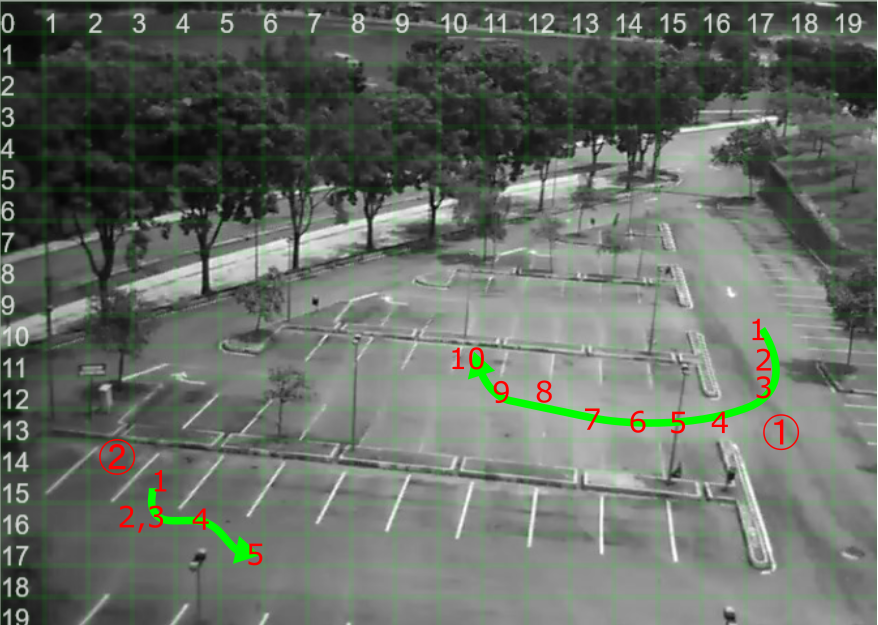
\includegraphics[width=.9\textwidth]{image/general/trajectorysample2.png}
\caption{Collection of a vehicle's centroids to represent the vehicle's motion}
\label{fig:motionExample}
\end{figure}
